\documentclass[11pt,a4paper]{jsarticle}
\usepackage[dvips]{graphicx}
\usepackage{fancyhdr}
\setcounter{page}{0}
%
\begin{document}

\title{制御工学実験II \\ 3.サーボモータのステップ同定}
\author{提出者 \\ 14104064 下松八重 宏太 \\ \\ 共同実験者 \\ 14101028 梶野 翔平 \\ 14104092 中島 美香 \\ 16104311 北山 拓夢 \\ 13104119 廣瀬 直人}
\date{実験日 2016年5月17日 \\ 提出日 2016年5月24日 \\ 再提出日 \today}



\maketitle
\thispagestyle{empty}
\newpage


\section{目的}
サーボモータを対象とし,制御対象の未知パラメータを同定するための1つの手段を習得することを主目的とする.また,対象を同定することがどのようなことなのかを理解する.

\section{原理}
本実験ではサーボモータにステップ状目標角度(一定電圧)を印加した時の円盤回転角度を計測することにより,入力電圧から目標角度までの伝達特性のパラメータを同定する.
  \subsection{対象の数学モデル}
  モータへの入力電圧$u$から円盤の回転角$\theta$までの伝達特性は
  \begin{equation}
  \it{\Theta} (s) = \frac{k}{Ts + 1} U(s)
    \label{eq1}
  \end{equation}
  で与えられている.ここで$U(s) = \frac{r}{s}$であり,$r$は目標角度である.このとき
  \begin{eqnarray}
   \it{\Theta(s)} & = & \frac{kr}{(Ts + 1)s}  \nonumber \\ 
    & = & kr(\frac{a_1}{Ts + 1} + \frac{a_2}{s})
    \label{eq2}
  \end{eqnarray}
  である.ここで,$a_1,a_2$は
  \begin{eqnarray*}
   a_1 & = & \lim_{s \to -\frac{1}{T}} (Ts + 1) \frac{1}{(Ts +1)s} = -T \\
   a_2 & = & \lim_{s \to 0} s \frac{1}{(Ts +1)s} = 1 
  \end{eqnarray*}
  となり,
  \begin{eqnarray*}
 \it{\Theta(s)} & = & kr(- \frac{T}{Ts + 1} + \frac{1}{s}) \\
& = & kr(- \frac{1}{s + \frac{1}{T}} + \frac{1}{s})
  \end{eqnarray*}
  である.$\it{\Theta(s)}$を逆ラプラス変換すると
  \begin{equation}
   \it{\theta(t)} = rk(1-e^{-\frac{1}{T} t})
    \label{eq3}
  \end{equation}
  となる.一般に対象の時定数$T$及びゲイン$k$は未知である.このパラメータ$T,k$がわかれば,対象を解析することが出来る.

  \subsection{ステップ応答を用いる同定方法}
   式\ref{eq1}で表現される制御対象にステップ入力電圧$U = \frac{r}{s}$($r$:目標角度)を印加したときの応答について,計算機棟を用いて対象の出力を計測する場合,離散的なデータ$\theta(ih) (i = 0,\cdots,n)$が収集されることになる($h:$サンプリング周期.本実験では0.01[s]).ここでは,この離散データから対象の未知パラメータ$T,k$を同定する手法を説明する.
   式\ref{eq1}の対象にステップ入力を印加したとき,出力は前述の通り
  \begin{equation}
 \it{\theta(t)} = rk(1-e^{-\frac{1}{T}t})
  \label{eq4}
  \end{equation}
  となる.ここで,$\Delta \theta(t) \equiv \theta(t + h_1)-\theta(t)$($h_1$:データ処理用サンプリング周期)で定義すれば,
  \begin{equation}
   \Delta \theta(t) = rk(1-e^{-\frac{h_1}{T}})e^{-\frac{1}{T}}
    \label{eq5}
  \end{equation}
  となる.さらに,$z(t) \equiv \ln \Delta \theta(t)$で定義すれば,
  \begin{equation}
   z(t) = -at+b, a = \frac{1}{T}, b = \ln(rk(1-e^{-\frac{h_1}{T}}))
   \label{eq6} 
  \end{equation}
  となる.すなわち,時間$t$と$z(t)$との関係(具体的には$a,b$の値)がわかれば,式\ref{eq6}より$T,k$を計算することが出来る.式\ref{eq4}から式\ref{eq6}の関係より,同定法は以下のようになる.
  \begin{enumerate}
   \item サンプリング周期$h$と目標角度$r$の値を定め,データ$\theta(ih) (i = 0,\cdots,n)$を収集する.
   \item データ処理用サンプリング周期$h_1$の値を定める.データ$\theta(ih)$より$z(ih)$を計算しプロットする.さらに,各点を通る直線を最小二乗法を用いて引く.
   \item 求めた直線の傾きと切片から式\ref{eq6}より,$T,k$を計算する.
  \end{enumerate}

 \section{実験方法}
 \begin{enumerate}
  \item データ収集用プログラムを起動し,使用法に従ってデータを収集する.なお,サンプリング周期を$h = 0.01$[s]とする.
  \item 得られたデータより以下の方法で時定数$T$,ゲイン$k$を同定する.ただし,取得するデータ数$n$の値を$n = 20$とする.
	\begin{itemize}
	 \item[(1)] データ処理用サンプリング周期を$h_1 = 0.01$[s]として,グラフを作成し,時定数$\tau$,ゲイン$k$を同定する.
	 \item[(2)] データ処理用サンプリング周期を$h_1 = 0.05$[s]として,グラフを作成し,時定数$\tau$,ゲイン$k$を同定する.
	 \item[(3)] データ処理用サンプリング周期を$h_1 = 0.10$[s]として,グラフを作成し,時定数$\tau$,ゲイン$k$を同定する.
	\end{itemize}
 \end{enumerate}

\section{結果}
 同定結果を表\ref{tab1},図\ref{fig3},\ref{fig4},\ref{fig5}に示す.
\begin{table}[hb]
 \begin{center}
  \caption{同定結果}
  \begin{tabular}[b]{|c||c|c|c|c|c|c|} \hline
   \multicolumn{1}{|c||}{時間[s]}
   & \multicolumn{2}{c|}{$h_1 = 0.01$[s]} 
   & \multicolumn{2}{c|}{$h_1 = 0.05$[s]}
   & \multicolumn{2}{c|}{$h_1 = 0.10$[s]} \\ \hline
   -  & $\Delta \theta(t)$[deg] & $z(t)$ & $\Delta \theta(t)$[deg] & $z(t)$ & $\Delta \theta(t)$[deg] & $z(t)$ \\ \hline \hline 
   0.01 & 0.96 & -0.041 & 4.26 & 1.45 & 8.04 & 2.08 \\ \hline
   0.02 & 0.84 & -0.174 & 4.08 & 1.41 & 7.74 & 2.05 \\ \hline
   0.03 & 0.84 & -0.174 & 4.02 & 1.39 & 7.62 & 2.03 \\ \hline
   0.04 & 0.78 & -0.248 & 3.96 & 1.38 & 7.44 & 2.01 \\ \hline
   0.05 & 0.84 & -0.174 & 3.90 & 1.36 & 7.26 & 1.98 \\ \hline
   0.06 & 0.78 & -0.248 & 3.78 & 1.33 & 7.08 & 1.96 \\ \hline
   0.07 & 0.78 & -0.248 & 3.66 & 1.30 & 6.90 & 1.93 \\ \hline
   0.08 & 0.78 & -0.248 & 3.60 & 1.28 & 6.72 & 1.91 \\ \hline
   0.09 & 0.72 & -0.329 & 3.48 & 1.25 & 6.54 & 1.88 \\ \hline
   0.10 & 0.72 & -0.329 & 3.36 & 1.21 & 6.42 & 1.86 \\ \hline
   0.11 & 0.66 & -0.416 & 3.30 & 1.19 & 6.24 & 1.83 \\ \hline
   0.12 & 0.72 & -0.329 & 3.24 & 1.18 & 6.12 & 1.81 \\ \hline
   0.13 & 0.66 & -0.416 & 3.12 & 1.14 & 5.94 & 1.78 \\ \hline
   0.14 & 0.60 & -0.511 & 3.06 & 1.12 & 5.76 & 1.75 \\ \hline
   0.15 & 0.66 & -0.416 & 3.06 & 1.12 & 5.70 & 1.74 \\ \hline
   0.16 & 0.60 & -0.511 & 2.94 & 1.08 & 5.52 & 1.71 \\ \hline
   0.17 & 0.60 & -0.511 & 2.88 & 1.06 & 5.46 & 1.70 \\ \hline
   0.18 & 0.60 & -0.511 & 2.82 & 1.04 & 5.34 & 1.68 \\ \hline
   0.19 & 0.60 & -0.511 & 2.70 & 0.99 & 5.22 & 1.65 \\ \hline
   0.20 & 0.54 & -0.616 & 2.64 & 0.97 & 5.04 & 1.62 \\ \hline
  \end{tabular}
 \label{tab1}
 \end{center}
\end{table}

\newpage

\begin{figure}[hbp]
 \begin{center}
  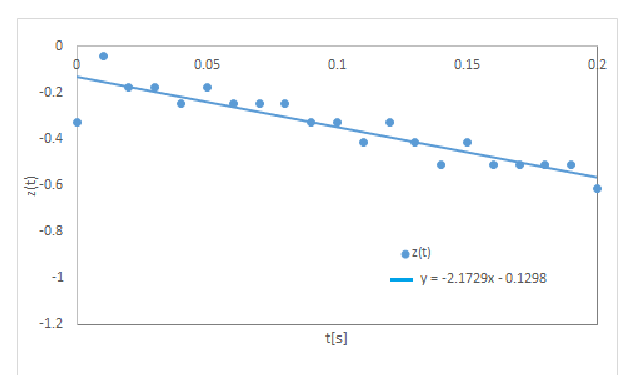
\includegraphics[scale = 1]{./picture/graph1.eps}
 \end{center}
 \caption{$h_1 = 0.01$[s]のときの$z(t)$}
 \label{fig3}
\end{figure}

\begin{figure}[hbp]
 \begin{center}
  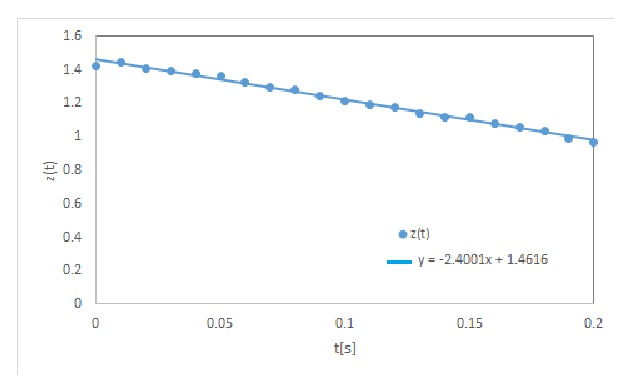
\includegraphics[scale = 1]{./picture/graph2.eps}
 \end{center}
 \caption{$h_1 = 0.05$[s]のときの$z(t)$}
 \label{fig4}
\end{figure}

\begin{figure}[htb]
 \begin{center}
  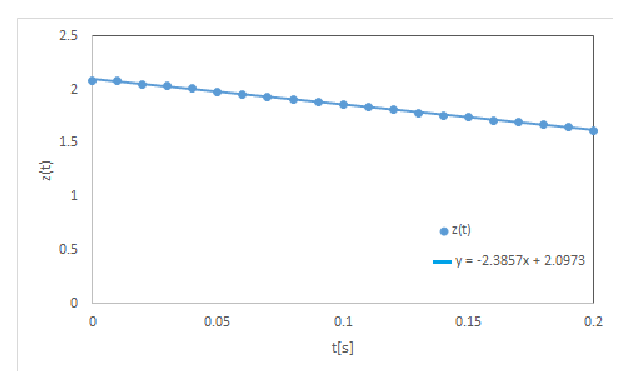
\includegraphics[scale = 1]{./picture/graph3.eps}
 \end{center}
 \caption{$h_1 = 0.10$[s]のときの$z(t)$}
 \label{fig5}
\end{figure}

\newpage

\section{考察}
式\ref{eq6}より$h_1 = 0.01,0.05,0.10$[s]についてそれぞれ$z(t)$を求めると
\begin{eqnarray}
 z(t) & = & -2.38t - 0.111 \\
 z(t) & = & -2.44t + 1.47 \\
 z(t) & = & -2.41t + 2.10 
\end{eqnarray}
となった.これより時定数$T$とゲイン$k$を求めると
\begin{eqnarray*}
 T = 0.420 & , & k = 0.845 \ (h_1 = 0.01[s]) \\
 T = 0.410 & , & k = 0.839 \ (h_1 = 0.05[s]) \\
 T = 0.414 & , & k = 0.846 \ (h_1 = 0.10[s]) \\
\end{eqnarray*}
となった.この$T$と$k$を用いて$\theta(ih)[deg] \ (i = 1,\cdots,20)$を求め,グラフにプロットすると図\ref{fig6}のようになった.

\begin{figure}[htb]
 \begin{center}
  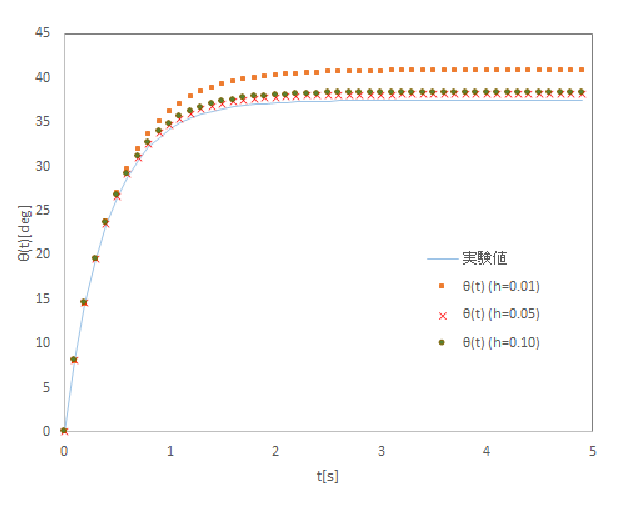
\includegraphics[scale = 1]{./picture/graph4.eps}
 \end{center}
 \caption{$\theta(t)$の実験値と同定結果}
 \label{fig6}
\end{figure}

\newpage

 \section{課題}
  \subsection{$\theta(t)$のグラフの比較}
   図\ref{fig6}より実験値と同定結果により得られた$\theta(t)$を比較するとその差は最大で3.41[deg],その時の相対誤差は9.2\%であった.また図\ref{fig6}より$h_1 = 0.05[s]$のとき最も精度よく同定できていることがわかる. \\
   どの同定結果も実験値とは一致していない.これは同定する際に使用した方程式にモデル化誤差が含まれているためである.また,最もサンプリング周期の高い$h_1 = 0.01[s]$のときより$h_1 = 0.05[s]$のときのほうが精度が良い.これには量子化誤差が影響していると考えられる.本実験では図\ref{fig3}よりサンプリング周期が高ければ高いほど$\Delta \theta(t)$の増加率が高い.これより$h_1 = 0.01[s]$のときより$h_1 = 0.05[s]$のときのほうが量子化誤差の影響が高いと考えられる.また,$h_1 = 0.10[s]$のときはサンプリング周期が大きすぎるために精度よく同定出来なかったと考える.

  \subsection{サーボモータとは}
   サーボモータとはサーボ機構を含むモータのことである.モータの回転角度をエンコーダ等によって計測し,これによってフィードバック制御を行うよう設計されている.

\newpage

\thispagestyle{fancy}
\rhead{再1}
\cfoot{}

\section{課題の補足}
\subsection{図\ref{fig3}について}
図\ref{fig3}において$t = 0.01,0.02$[s]のとき,近似直線から大きくずれた値になっている.これは本実験における数学モデルを1次遅れ系として同定している.しかし,本来は2次遅れ系であり,近似する際にフィードバックゲインを$0 < f_a << 1, f_b \simeq 1$として近似している.これより0に近い時間においては近似の影響が無視できず,同定結果に影響が表れたと考える.

\subsection{$\theta(t)$のグラフの比較}
モデル化誤差とはある物理現象を数式でモデル化した際に生じる誤差で,どの数式モデルにおいても生じる.本実験では入力電圧から回転角度までをモデル化している.また,量子化誤差とはアナログ信号を離散化する際にその値を近似することで生じる誤差である.図\ref{fig6}において$h_1 = 0.01$[s]の時より$h_1 = 0.05$[s]の時のほうが精度が向上しているのは前述の近似の影響があると考えられる.つまり,$h_1 = 0.01$[s]において$t = 0.01,0.02$[s]の時の値を除いて同定を行えば,精度よく同定出来ると考えられる.

\section{まとめ}
ステップ応答を用いる同定方法についてその手法を修得することが出来た.また,同定する際における誤差について理解することが出来た.

\newpage
\thispagestyle{fancy}
\rhead{再々1}
\cfoot{}

\setcounter{section}{3}
\section{実験結果}
同定結果のグラフを以下に示す.

\begin{figure}[htb]
 \begin{center}
  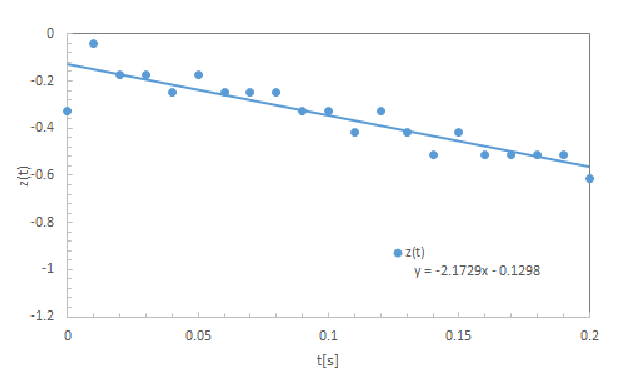
\includegraphics[scale = 1]{./picture/graph1_re.eps}
 \end{center}
 \caption{$h_1 = 0.01$[s]のときの$z(t)$}
\end{figure}

\begin{figure}[htb]
 \begin{center}
  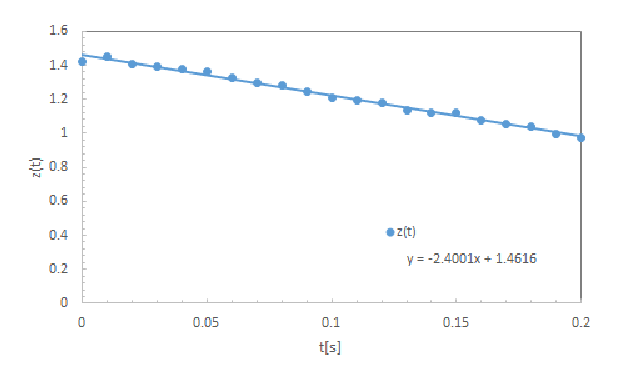
\includegraphics[scale = 1]{./picture/graph2_re.eps}
 \end{center}
 \caption{$h_1 = 0.05$[s]のときの$z(t)$}
\end{figure}

\newpage
\thispagestyle{fancy}
\rhead{再々2}
\cfoot{}

\begin{figure}[htb]
 \begin{center}
  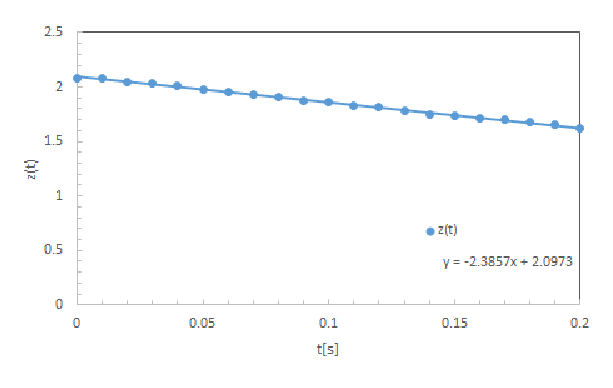
\includegraphics[scale = 1]{./picture/graph3_re.eps}
 \end{center}
 \caption{$h_1 = 0.10$[s]のときの$z(t)$}
\end{figure}

\begin{figure}[htb]
 \begin{center}
  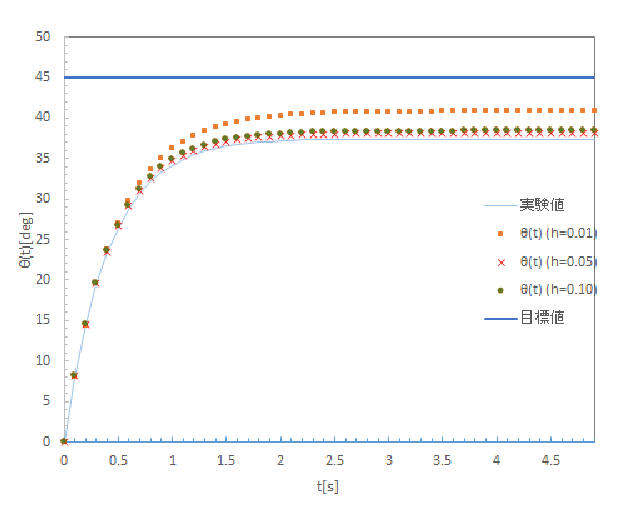
\includegraphics[scale = 1]{./picture/graph4_re.eps}
 \end{center}
 \caption{$\theta(t)$の実験値と同定結果}
\end{figure}

\newpage
\thispagestyle{fancy}
\rhead{再々2}
\cfoot{}


\newpage
\thispagestyle{fancy}
\rhead{再々3}
\cfoot{}


\setcounter{section}{6}
\section{課題の補足}
\subsection{図\ref{fig3}について}
図\ref{fig3}において$t = 0.01,0.02$[s]のとき,近似直線から大きくずれた値になっている点について,この制御系は非線形性を有している.このとき,制御系は不感帯特性を示す.印加電圧が小さいとき,モータは摩擦力によって動き出さず,ある値を超えたときに動き出す.図$\ref{fig3}$の$t = 0.01,0.02$[s]のときはこの不感帯であったと考えられる.また,非線形制御系ではヒステリシス特性を持つ.機構にがたがある場合に入力方向が逆になったとき,一時的にその位置を保ち,そこから逆方向に動き出す.サンプリング周期が短い場合,このヒステリシス特性によるばらつきがグラフに表れていると考えられる.

\subsection{$\theta(t)$のグラフの比較}
図\ref{fig6}においてサンプリング周期が短すぎても長すぎても同定精度が低くなっている.よってサンプリング周期は短すぎず長すぎない適当な値を選択する必要がある.


\newpage
\thispagestyle{fancy}
\rhead{再々々1}
\cfoot{}

\setcounter{section}{3}
\section{実験結果}
同定結果のグラフを以下に示す.

\begin{figure}[htb]
 \begin{center}
  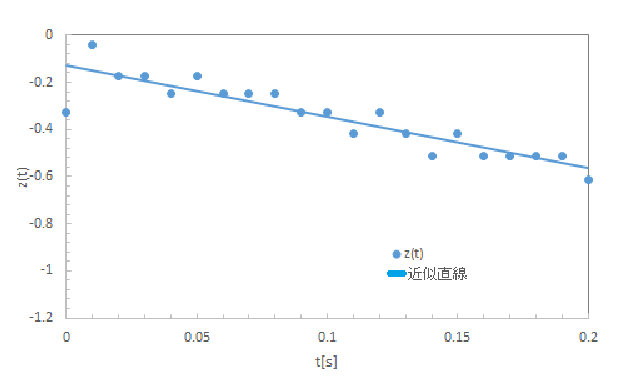
\includegraphics[scale = 1]{./picture/graph1_re2.eps}
 \end{center}
 \caption{$h_1 = 0.01$[s]のときの$z(t)$}
\end{figure}

\begin{figure}[htb]
 \begin{center}
  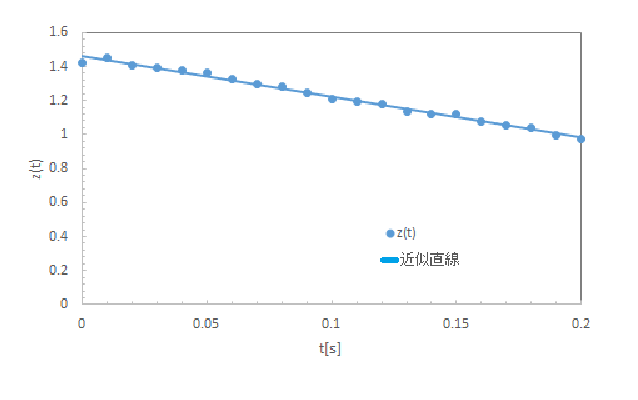
\includegraphics[scale = 1]{./picture/graph2_re2.eps}
 \end{center}
 \caption{$h_1 = 0.05$[s]のときの$z(t)$}
\end{figure}

\newpage
\thispagestyle{fancy}
\rhead{再々々2}
\cfoot{}

\begin{figure}[htb]
 \begin{center}
  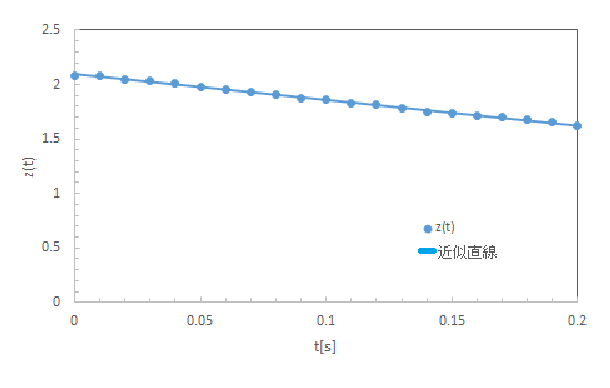
\includegraphics[scale = 1]{./picture/graph3_re2.eps}
 \end{center}
 \caption{$h_1 = 0.10$[s]のときの$z(t)$}
\end{figure}


\end{document}








